\documentclass[a4paper,notitlepage,11pt]{article}
\usepackage[dvipsnames]{xcolor}
\usepackage{tikz}
\usetikzlibrary{calc}
% add bulgarian support
\usepackage[utf8]{inputenc}
%\usepackage[english,bulgarian]{babel}
%\usepackage[T2B]{fontenc}
\usepackage[a4paper, total={7.5in, 10.5in}]{geometry}
\usepackage[most]{tcolorbox}
\usepackage{tikz,lipsum,lmodern}
\usepackage{mymacros}
\usepackage[backref=true,                % 
            hyperref=true,               % 
            firstinits=true,             %
            indexing=true,               %
            url=false,                   % 
            style=alphabetic,            %  style=debug, alphabetic
            bibstyle=ieee,               %
            backend=biber,               % 
            doi=true,
            texencoding=utf8,
            bibencoding=utf8]{biblatex}
\addbibresource{myPublications.bib}
\begin{document}
% turn off page numbering
\thispagestyle{empty}

\definecolor{myblue}{rgb}{0.0,0.7,1.0}
\definecolor{mylightblue}{rgb}{0.0,0.1,1.0}
\begin{figure}[t!]
  \hspace{-2cm}
%  \centering
\begin{tikzpicture}
   \coordinate (BL) at (-3,0);
   \coordinate (TR) at (19,3);

   \coordinate (A)  at (8,2.2);
   \coordinate (D)  at (8.8,3);

   \coordinate (A2) at (-3,2.2);
   \coordinate (B)  at (10.2,0);
   \coordinate (C)  at (11,0.8);
   \coordinate (C2) at (19,0.8);

%   \draw[step=1cm,gray,very thin] (BL) grid (TR);
   \draw[myblue, fill=myblue] (BL)--(B)--(A)--(A2)--cycle;
   \draw[myblue, fill=myblue] (C)--(D)--(TR)--(C2)--cycle;
   \draw[myblue, fill=myblue] (0,0.5) rectangle (2.7,3.5);
%   \draw[mylightblue, fill=mylightblue](A)--(B)--(C)--(D)--cycle;
%   \draw[myblue, fill=myblue] at (3.0, 0.0) rectangle (2.5cm, 3.0cm);
   \node[anchor=south west,inner sep=0] at (0.1,0.5) {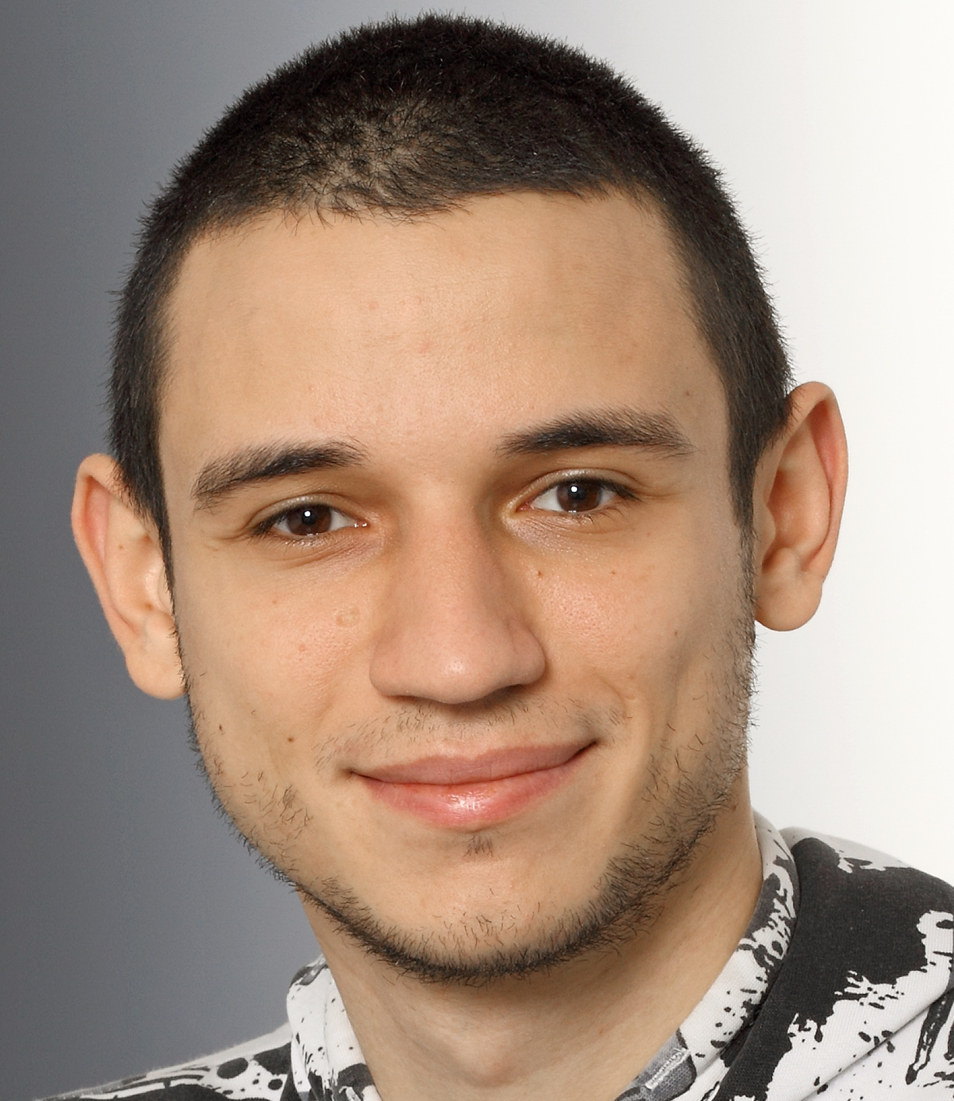
\includegraphics[width=2.5cm]{../ymadzhunkov.jpg}};
   \node[draw=none,align=left] at (5.8,1) {
      \color{white}\Large \textbf{Yordan Madzhunkov}\\ 
      \color{white}Physicist, Software Developer\\
      \color{white}ymadzhunkov@gmail.com
   };
   \node[draw=none,align=left] at (14.5,2) {
      \color{white} \large \textbf{"Creativity is intelligence having fun"}\\ 
      \color{white}  \quad \quad \quad \quad \quad \quad \quad \quad Albert Einstein
   };
\end{tikzpicture}



\end{figure}
\noindent
\begin{minipage}[t]{.6\textwidth}
      % “Everything must be made as simple as possible. But not simpler.” 
%\mysection{Summary}
I am looking for a good manager of a highly paid team that is solving
interesting problems for real people. I have strong background in math, physics
and software development. I have 12+ years of experience with C++. I value well
crafted code. For me responsibility is always personal.\\
Compensation Expectations: Net 9000+ BGN per month 
\mysection{Top Employers}
\myjobb
{2017--present}
{Computer Vision Engineer}
{Alcatraz AI}
{Sofia, Bulgaria}
{
\item Validate and adapt ML models
\item Data collection
}
{
\item Application development
\item Interview engineers 
}
{CMake, C++14, python, bash}
\myjobb
{2016--2017}
{Software Cleaner}
{Viewray}
{Sofia, Bulgaria}
{
\item Automated deployment 
\item Automated testing 
}
{
\item Removed over 40 \% of the code base ( dead code ) 
}
{CMake, bash, gcov}
\myjobb
{2016--2016}
{Machine learning engineer}
{HyperScience}
{Sofia, Bulgaria}
{
\item Machine learning 
}
{
\item 3 prototypes in 5 months
}
{clojure, python, sklearn}
\myjobb
{2014--2016}
{Software Developer}
{Chaos Group}
{Sofia, Bulgaria}
{
\item Optimized V-Ray hair shading
\item Improved CMake build system 
\item Improved precision in Embree and V-Ray
}
{
\item Integrated Embree library in V-Ray $\Rightarrow$ 10\% better render times 
\item Improved Embree hair intersection 
\item Involved in company public image
}
{C++, algorithms, multithreaded, computer graphics, CMake, code reviews, git, intrinsics, refactoring, unit tests}
%\myjobb{2011--2014}
%{Algorithm Developer}
%{Rheinisch-Westfälische Technische Hochschule}
%{Aachen, Germany}
%{
% \item Implemented parallel SVD
% \item Image processing algorithm
%}
%{
%\item Automatic collection of data from simulations on Blue Gene/Q
%}
%{C++, multithreaded, MPI, computational algebra, raytracing, git, \LaTeX, mathematical optimization}
%\myjobbb{2010--2011}
%{Algorithm developer}
%{MM Solutions}
%{Sofia, Bulgaria}
%{ \item Developed algorithms for digital video stabilization project}
%{C++, image processing, pattern recognition, statistics beyond the university level}
\myjobb{2006--2010}{Student Research Assistant}
{Dosimetry and Rad. Protection, Sofia University} {Sofia, Bulgaria}
{
 \item Co-author of 9 papers
 \item Developed software for automation of experiments
}
{ 
 \item Gathered, analysed and visualized data from Monte Carlo simulations on supercomputers
}
{C/C++, Pascal, Fortran, Linux, Monte Carlo, High Performance Computing}


\end{minipage}% This must go next to `\end{minipage}`
\quad
\quad
\fcolorbox{myblue}{myblue}{
\begin{minipage}[t]{.39\textwidth}
\color{white}
%%%%%%%%%%%%%%%%%%%%%%%%%%%%%
%   P R O G R A M M I N G   %
%%%%%%%%%%%%%%%%%%%%%%%%%%%%%
%\myskillset{Programing skills}{
%\item Algorithms
%\item Parallel
%\item Design Patterns
%\item Refactoring 
%}
%{
%\item Data Structures
%\item Unit Testing
%\item Object Oriented 
%\item Optimization
%}
%\vspace{-0.8cm}
%\mysection{Programing Languages}
%Favorite: C/C++\\
%Worked with: Assembler, bash, make, \LaTeX, Pascal, Fortran, OpenMP, MPI, CMake, clojure, Java, C\#, php, python, perl, Matlab, Mathematica
%\vspace{-0.4cm}
\mysection{Favorite programing environment}
C++, CMake, GNU/Linux, vim, clang, gcc
\mysection{Adopted Development Practices}
\begin{tabular}{ l l}
 Test Driven Development & Code Reviews \\
 Continuous Refactoring & Style guide \\
 Continuous Integration & Testing \\
\end{tabular}\\
%\mysection{Passionately curious about}
%"I have no special talents. I am only passionately curious."\\
%\hfill Albert Einstein\\
%\begin{tabular}{ l l}
%Physics             & Numerical Methods         \\
%Monte Carlo         & Computer Simulations     \\ 
%Computer Vision     & Image processing          \\
%Sparse Matrices     & Probability \& Statistics \\
%Linear Algebra      & Pattern Recognition      \\   
%Modeling Data       & Optimization              \\
%Psychology          & Sociology \\
%\end{tabular}\\
\vspace{-0.4cm}
\mysection{Top 4 Awards in Physics}
\begin{tabular}{ p{0.1\textwidth} p{0.18\textwidth} p{0.50\textwidth} }
year & award & Competition \\
\hline
2006 & Silver  & Intenational Physics \\
     & Medal   & Olympiad, Singapore  \\
2006 & Laureate& National Olympiad\\
2006 & I   & Special Class, Plovdiv  \\
2005 & I   & Special Class, Ruse     \\
\end{tabular}\\
\vspace{-0.4cm}
\mysection{Top 4 Awards in Informatics}
\begin{tabular}{ p{0.1\textwidth} p{0.18\textwidth} p{0.50\textwidth} }
year & award & Competition \\
\hline
2006 & Laureate  & National Olympiad \\
2005 & II        & Class B \\
2003 & I         & Class B, Yambol \\
2007 & II        & codeit (MusalaSoft)\\
\end{tabular}\\
\vspace{-0.4cm}
\mysection{Conferences}
Code for Art 2016 - Test Driven Development \\
Code for Art 2015 - Monte Carlo Method \\
Code for Art 2014 - Embree in V-Ray\\
\vspace{-0.4cm}
\mysection{Top 3 Scholarships}
2011 - DAAD Master degree in Germany \\
2009 - Development of egs\_pet code \\
2006 - Evrika Foundation - Medal IPhO\\
\vspace{-0.4cm}
\mysection{Languages}
\begin{tabular}{ l l }
Bulgarian & Mothertongue \\
English   & Fluent, TOEFL 107/120\\
\end{tabular}\\

\end{minipage}
}
\newpage
\thispagestyle{empty}
\noindent
\begin{minipage}[t]{.6\textwidth}
   \vspace{0.1cm}
   \myjobbb{2013--2014}
{Algorithm Developer}
{Computational Engineering Science, RWTH}
{Aachen, Germany}
{ \item Implemented scalable parallel singular value decomposition with multiple relatively robust representations}
{C++, multithreaded programing, numerical stability, unit testing, git, \LaTeX}
\myjobb{2012--2013}
{Student Research Assistant} 
{Process Engineering Department, RWTH}
{Aachen, Germany}
{ \item Researched image processing algorithm to collect valuable experimental data}
{ 
%\item Provided valuable insight to project
\item Developed proof of concept algorithm and developed simulator to validate it}
{C++, computer graphics, linear algebra, sparse matrices, raytracing, mathematical optimization}
\myjobb{2011--2012}
{Student Research Assistant}
{Parallel Programing Lab, RWTH}
{Aachen, Germany}
{\item Simulations on Blue Gene/Q}
{\item Developed a tool to process data}
{ C++, MPI, bash, xml, parsing}
\myjobbb{2010--2011}
{Algorithm developer}
{MM Solutions}
{Sofia, Bulgaria}
{ \item Developed algorithms for digital video stabilization project}
{C++, digital image processing, pattern recognition, statistics beyond the university level, testing}
\myjobbb{Summer 2008}{Software Consultant}
{Scopic Software, Rutland MA, USA}{Sofia, Bulgaria}
{\item Maintained Image Processing Software}
{C\#, digital image processing, pattern recognition, classification algorithms, workflow with quality assurance}
\myjobb{2006--2010}{Student Research Assistant}
{Dosimetry and Rad. Protection, Sofia University} {Sofia, Bulgaria}
{
 \item Involved in scientific projects 
 \item Co-author of 9 papers
 \item Developed software for automation of experiments
}
{ 
 \item Developed Monte Carlo for Positron Emission Tomography
 \item Gathered, analysed and visualized data from supercomputers
}
{Linux, C/C++, Pascal, Fortran, OOP, Design Patterns, Monte Carlo, Revision control, High Performance Computing and many more}
\vspace{-0.8cm}
\mysection{Personality Strengths}
\small
\textbf{Critical Thinker} - I enjoy to analyze problems from every angle in quest for best solutions. I easily use my accumulated knowledge to identify fallacious arguments and systematical contradictions. Therefore, I can produce factual knowledge that can be trusted.\\
\textbf{Knowledgeable} - I rarely pass up to learn something
new. I just find it fun and fascinating.\\
\textbf{Original and Energetic} - If presented with chronic, systemic
problems, I respond with enthusiasm and energy, putting days and nights to find a solution.\\
\textbf{Excellent Brainstormer} - I am confident in my abilities. I
have passion to share my opinion, knowledge and critical thinking with my colleagues.\\
\textbf{Charismatic} – People find intriguing my way with words. My confidence, quick thought and ability to connect distant ideas in novel ways create a style of communication that is charming, entertaining, and informative at the same time.\\
\textbf{People Master} - I have very good communication skills, feeling at ease in social events or in situations where I need to connect to other people. Playing an active role in the society and knowing what makes other people tick means a lot for me. However, I am not influenced easily by others opinion about me.



\end{minipage}% This must go next to `\end{minipage}`
\quad
\quad
\fcolorbox{myblue}{myblue}{
\begin{minipage}[t]{.39\textwidth}
\color{white}
\mysection{Awards in Physics}
\begin{tabular}{ p{0.1\textwidth} p{0.18\textwidth} p{0.50\textwidth} }
year & award & Competition \\
\hline
2006 & Silver  & Intenational Physics \\
     & Medal   & Olympiad, Singapore  \\
2006 & Laureate& National Olympiad\\
2006 & I   & Special Class, Plovdiv  \\
2005 & I   & Special Class, Ruse     \\
2004 & III   & Special Class, Pleven   \\
2003 & II  & 10 grade, St. Zagora  \\
2003 & III   & 9 grade,  Kovachevtsi   \\
2002 & I   & 9 grade,  Botevgrad     \\
2001 & I   & 8 grade,  Turnovo\\
\end{tabular}\\
\vspace{-0.4cm}
\mysection{Awards in Informatics}
\begin{tabular}{ p{0.1\textwidth} p{0.18\textwidth} p{0.50\textwidth} }
year & award & Competition \\
\hline
2006 & Laureate  & National Olympiad \\
2005 & II        & Class B \\
2003 & I         & Class B, Yambol \\
2003 & III       & Class B \\
\end{tabular}\\
\vspace{-0.4cm}
\mysection{Online Programming Contest}
\begin{tabular}{ p{0.1\textwidth} p{0.10\textwidth} p{0.58\textwidth} }
year & award & Competition \\
\hline
2007 & II    & PC Magazine, MusalaSoft and BASSCOM \\
2006 & II    & Magazine "Computer"\\
\end{tabular}\\
\vspace{-0.4cm}
\mysection{Scholarships}
2011 - DAAD Master degree in Germany \\
2009 - Development of egs\_pet code \\
2007 - Positron Emission Tomography\\
2006 - Evrika Foundation - Medal IPhO\\
\vspace{-0.4cm}
\mysection{Languages}
\begin{tabular}{ l l }
Bulgarian & Mothertongue \\
English   & Fluent, TOEFL 107/120\\
\end{tabular}\\

\end{minipage}
}
%\newpage
%\section*{Bibliographies}
%\nocite{*}
%\printbibliography
\end{document}

